\documentclass{article} % For LaTeX2e
\usepackage{nips14submit_e,times}
\usepackage{graphicx}
\usepackage{hyperref}
\usepackage{url}
%\documentstyle[nips14submit_09,times,art10]{article} % For LaTeX 2.09


\nipsfinalcopy
\title{Employing an HMM and Decision Tree to Predict Student Behavior}

\author{
Maximo Q.~Menchaca\\
Department of Atmospheric Science\\
518 ATG\\
\texttt{menchaca@uw.edu} \\
\And
John G.~Lee\\
Department of Physics \\
180 NPL Building \\
\texttt{jgl6@uw.edu} \\
}

% The \author macro works with any number of authors. There are two commands
% used to separate the names and addresses of multiple authors: \And and \AND.
%
% Using \And between authors leaves it to \LaTeX{} to determine where to break
% the lines. Using \AND forces a linebreak at that point. So, if \LaTeX{}
% puts 3 of 4 authors names on the first line, and the last on the second
% line, try using \AND instead of \And before the third author name.

\newcommand{\fix}{\marginpar{FIX}}
\newcommand{\new}{\marginpar{NEW}}

%\nipsfinalcopy % Uncomment for camera-ready version

\begin{document}

\maketitle

\begin{abstract}
An online tutoring system tracks student interactions as they learn. The tracked interactions can be used to predict future student performance. A decision tree and a Hidden Markov Model (HMM) were used in conjunction to determine the learning rate of a student. Output from the decision tree determined that the step duration provided valuable information gain on the training data. Within this paper, we develop a decision tree that splits on both the step duration and opportunity of the skill involved in the step to predict the probability a student achieves a first correct on a given problem. A Hidden Markov Model is used to predict the expected step duration at a given test data point, which is then plugged into the decision tree.
\end{abstract}

\section{Introduction}
This project was developed from the 2010 KDD Cup Challenge. The challenge is based off a database of student interactions with an online Cognitive Tutors system. The challenge specifically provides us with 5 high school level algebra datasets. These datasets are extremely large, with some containing thousands of students and 20 million total interactions. Within, each step the student encounters is logged. Associated with each step is the time spent, the problem unit, section, and name, the skill associated with this step, the number of times a student has encountered the relevant skill (called the "Opportunity"), and student queries. Either (1) the student does not know how to do the problem and asks for help (Hints), (2) the student inputs an incorrect answer (Incorrects), or (3) the student inputs a correct answer (Corrects). The goal of the challenge is to use the training portions of the dataset to predict whether or not a student will achieve a "Correct" on their first attempt at a step given in the test set, i.e., the first interaction of a student with a particular step is a "Correct" rather than a "Hint" or "Incorrect".

At face value, an intuitive structure to developing a successful algorithm is not difficult. As students progress through the dataset, one would expect the students to generally improve at their algebra skills throughout the year. If we expect students to do better later on in the year than earlier, the temporal nature of the data must be taken into account. Given the time series nature of the data, a Hidden Markov Model (hereafter HMM) seems a natural choice to generate predictions of student performance.

One could then develop an HMM that shows improving performance with time, and from this develop probabilities of getting a "First Correct". However, the dataset is not conducive to such a simple system.

\section{Proposed Methods}

\subsection{Hidden Markov Model}

A Hidden Markov Model is a time series where the states of the underlying system are unknown, or 'hidden'. For example, a dishonest casino could occasionally switch a fair die for a loaded die, and the goal of the unlucky gamblers is to determine when the casino has performed the switch. This involves determining (1) the probability a round of gambling has started with the fair or loaded die (the STARTING probability of each state), (2) the probability that the die are being switch (the TRANSITION probability of each state), and (3) the probability of each output from the die in each state (the EMISSION probability of each state). In the example above, a fair die would have an equal $\frac{1}{6}$ chance of emitting a 1,2,3,4,5,6, while the loaded die would have, say, a $\frac{1}{2}$ of rolling a 3.

In the problem we are considering for this paper, we hope to develop hidden states relating to the student's comprehension. This seems fitting, as we can see in Figure \ref{learning_curve}. This figure depicts the fraction of "First Corrects" as a function of the Opportunity - in other words, the plotted value for the x value of 1 would be the fraction of "First Corrects" the first time ALL students encounter a given skill, an x value of 2 the fraction of "First Corrects" the SECOND time all students encountera given skill, etc... As we can see, this plot rapidly increases, but then thresholds near a value of 0.8. This learning curve prompts us to develop a template HMM with three hidden states: "Unknowledgeable", "Learning", and "Comprehension". From these hidden states, we emit the probability of getting a problem first correct - higher for higher states of comprehension. A possible blueprint is shown in Table \ref{HMMprop}.

\begin{figure}[h]
\begin{center}
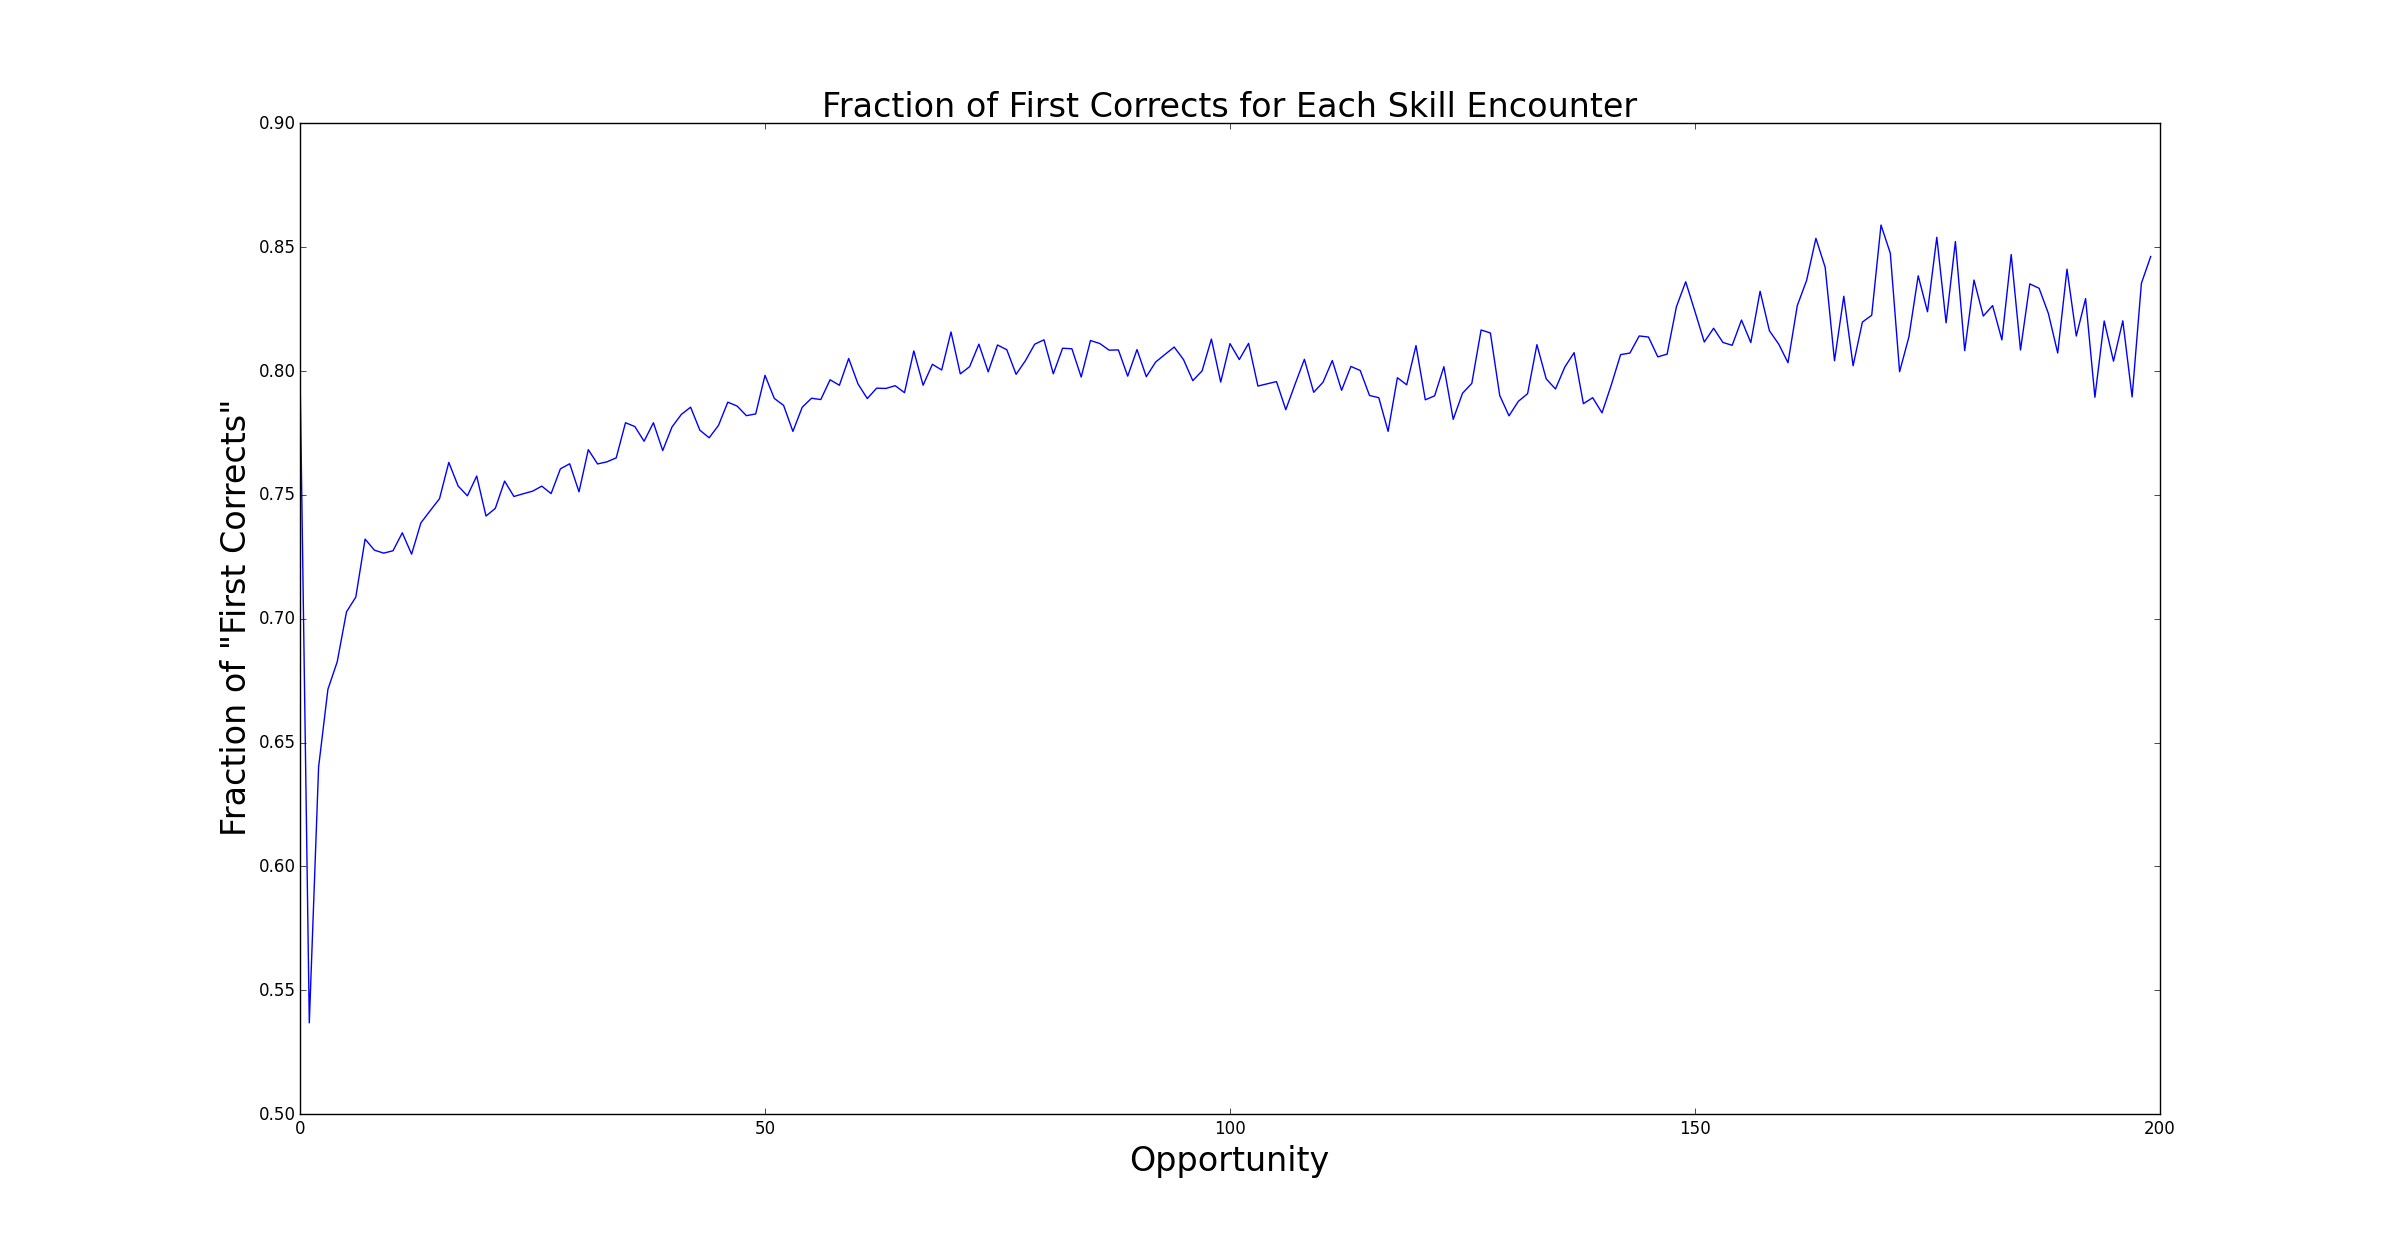
\includegraphics[width=0.8\textwidth]{fracCORR_opp.png}
\label{learning_curve}
\end{center}
\caption{Fraction of "First Corrects" as a function of opportunity, demonstrating a "learning curve".}
\end{figure}


\begin{table}[t]
\begin{center}
\begin{tabular}{ccc|c|ccc|cc}
\multicolumn{3}{c}{$\pi$} && \multicolumn{3}{c}{$T$} & \multicolumn{2}{c}{$E$}\\
UK & L & C & & UK & L & C & 0 & 1\\
& & & UK &0.8 & 0.2 & 0.00  & 0.6 & 0.4\\
1.0 & 0.0 & 0.0 & L & 0.02 & 0.85 & 0.13 & 0.45 & 0.55\\
&&& C & 0.01 & 0.01 & 0.98 & 0.15 & 0.85\\

\end{tabular}
\caption{A proposed Hidden Markov Model for a student's learning history.}\label{HMMprop}
\end{center}
\end{table}

In the template HMM shown, we expect to start in the "Unknowledgeable" state, which has a 40\% chance of getting a 0. However, the student progresses to the "Learning" state as they progress, which hives us a higher chance (55\%) of getting the problem first correct. Finally, the student progresses to the terminal "Comprehension" state. The transition and emission probabilities in the template could be modified upwards or downwards depending on the speed at which the student learns.

\subsection{Forward-Backward Test}
A hidden Markov model (HMM) was initially implemented to track the learning curve of the individual students and predict subsequent observable features [1]-[2]. We assumed a hidden state tracked whether the student was knowledgeable or not at the time i in order to predict the probability of getting the problem i+1 correct on the first attempt. The model required the creation of a finite set of possible observations given the various preprocessed variables. 

We first experimented with smoothing by applying the forward-backward algorithm to predict subsequent Correct First Attempt variables, using educated but rough assumptions about $\pi$, $T$, and $E$ of the hidden and observed states. The smoothed data then predicted a probability for observing the next Correct on First Attempt variable as a 1 [6].

The output probabilities were greatly affected by underflows and many states were non-predictive. Our implementation of the forward-backward algorithm was improved by introducing rescalings to prevent underflows [5]. A few quick tests were performed stepping through different transition probabilites from the unknowledgeable state, see figure~\ref{fig:dunno}. This motivated us to attempt to train the HMM parameters. The implementation of the forward-backward algorithm was necessary for eventually predicting features for the test data.

\begin{figure}[h]
\begin{center}
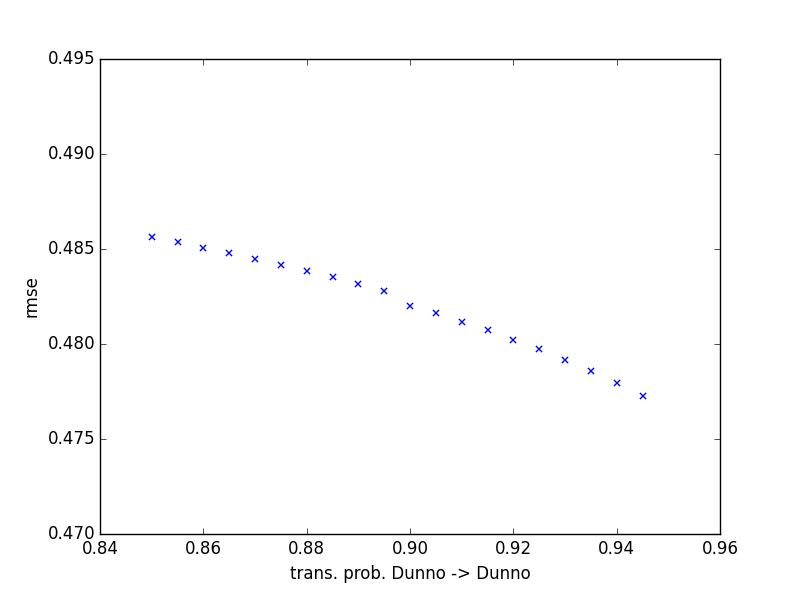
\includegraphics[width=0.8\textwidth]{dunno.png}
\label{fig:dunno}
\end{center}
\caption{Root-Mean-Square-Error with increasing probability of staying at unknowledgeable state from problem to problem.}
\end{figure}

\subsection{Baum-Welch}
With a working implementation of the forward-backward algorithm we then set to work developing the Baum-Welch algorithm. The algorithm is an implementation of Expectation Maximization. Current hidden variable states are estimated through the forward-backward algorithm and then state transitions and observations are counted to update $\pi$, $T$, and $E$. The algorithm is typically meant to be employed over long time series of data which our data sets did not necessarily provide. Instead we implemented a Stochastic Gradient Descent type update, by iterating over short time series of multiple students and averaging, see ~\ref{fig:sgdbw}.

With the Baum-Welch algorithm, we developed a set of general model parameters ($\pi$, $T$, and $E$) which were applied in the forward-backward algorithm on each student to predict features in the test data. In a sense, this served as our model of how a student learns through time, and the individual time series of student questions updated model of how much the student knew at a given time.

\begin{figure}[h]
\begin{center}
	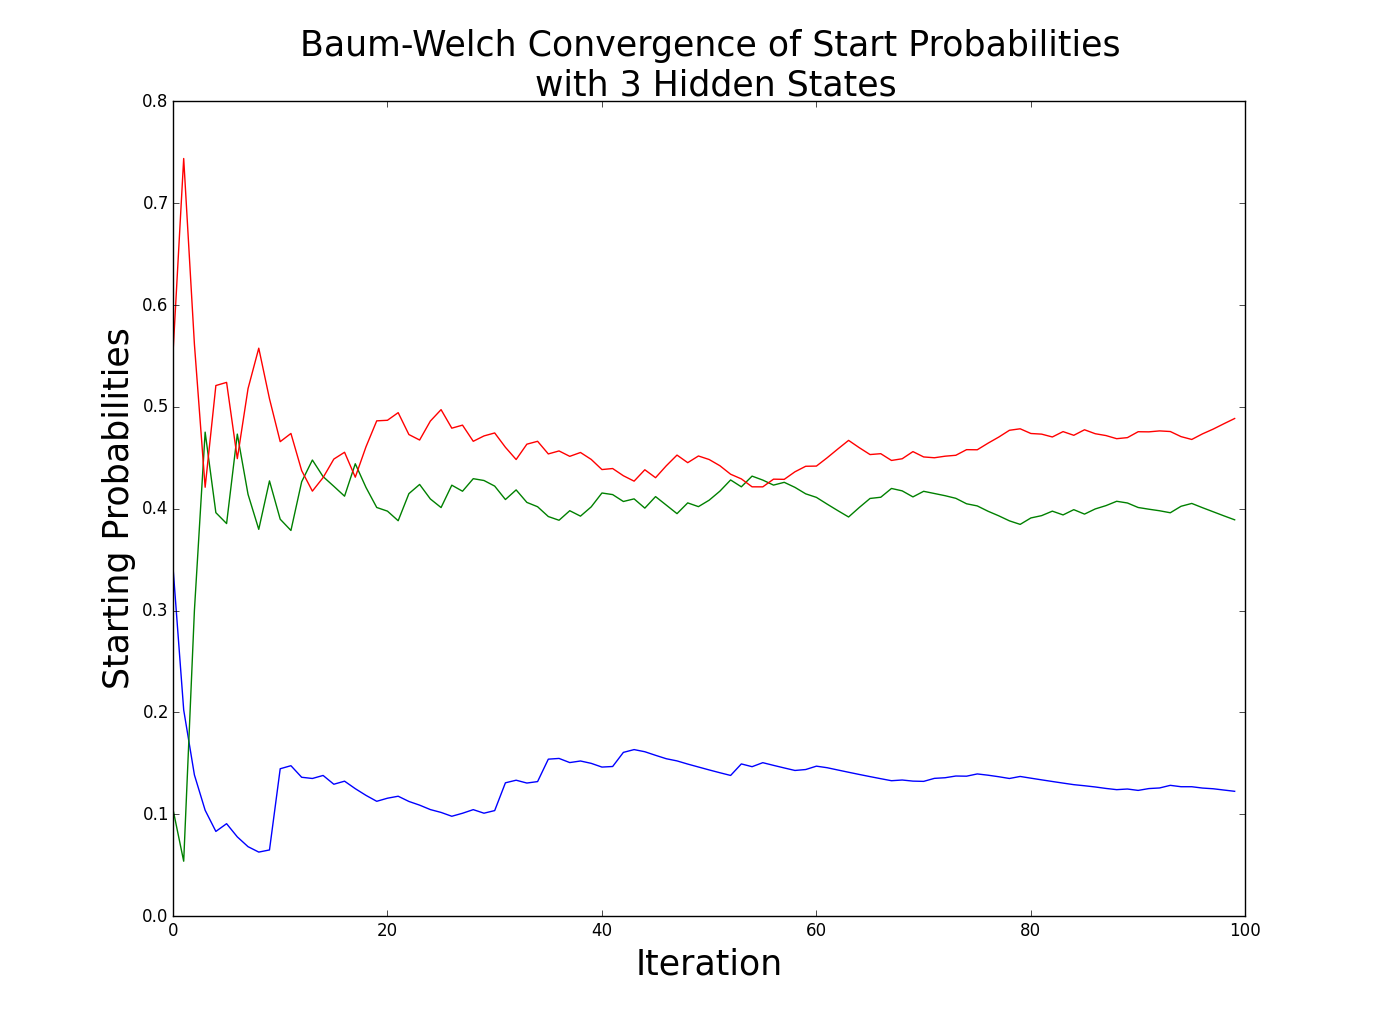
\includegraphics[width=0.8\textwidth]{bwConv3a.png}
	\label{fig:sgdbw}
\end{center}
\caption{Example of convergence of Baum-Welch algorithm over 100 students}
\end{figure}

\subsection{Limitations to the Naive Approach}

Of course, there are numerous obstacles to the methods described in this template. Ideally, one could adapt this rough blueprint to each student and skill, creating $T$ and $E$ matrices that allow us to predict student behavior. However, the data is sparse. Not all students see all skills. As a matter of fact, some students have as few as 12 data points total in the training datset. Even worse, students exist in the test set that are NOT in the training set. Similarly, there are skills that are present in the test subset that never appeared during training. Evidently, with new features in the test set, creating an HMM specific to each student and skill is a pipe dream.

A further limitation arises due to the binary nature of our predicted variable, "Correct First Attempt". Given two possible emissions, a naive model built to predict this variable could give us two possible hidden states (the third of Table \ref{HMMprop} would be superfluous) - "Correct" and "Incorrect". Where "Correct First Attempt" is 1, we must be in the "Correct" state, while if "Correct First Attempt" is 0, we must be in the "Incorrect" state. Such output is useless for application to our test data!

There are numerous other limitations inherent to our data set. The Markov Model assumption relies on data being sequential - something that is not necessarily true in our training data. Numerous gaps exist, and should be taken into account. And most frustratingly, much of the information associated with a step is not present in the test data at all - we are only given the "Opportunity", row in the full dataset, and problem name. We therefore must find a variable related to "Correct First Attempt" in order to provide more robust output from the Baum-Welch algorithm in developing our HMM.

\subsection{Decision Tree}
In order to find a variable that provides a prediction of "Correct First Attempt", we turn to decision trees and the concept of entropy. The entropy of a dataset is defined as
$$
H(Y) = -\sum_{i=1}^k P(Y = y_i) log P(Y = y_i),
$$
where we sum over all the classes $y_i$ of the output/dependent variable $Y$. For the smallest data set we have, Algebra I 2005-2006 (the training data set has about 800,000 members), the base entropy is $H(Y) = 0.79$. Do any of the independent variables provide an information gain for "Correct First Attempt"? Obviously, variables like "Hints" or "Incorrects" will be poor predictors of "Correct First Attempt", as only zero values of the former can lead to the latter being 1.

It is also likely that the Problem Hierarchy - the Unit, Section, and Name - could influence the likelihood of a student achieving a correct on the first try. Surely, some problems are more difficult than others. In our smallest dataset, there are 33 unique problem units, and 136 problem sections. Overview of the variance of the fraction of "Correct First Attemps" for the unique problem units and sections reveals a spread ranging from 0.68 to 0.81. We have chosen to NOT split on these variables, for a variety of reasons. First, they would partition the dataset into smaller chunks, increasing the complexity of the decision tree, while reducing the number of data samples with which to train our algorithm. Second, as mentioned above, our dataset is sparse - not all students see all units and sections. Employing the problem information to inform our algorithm may be worth the effort if it comes at the payoff of much better prediction. However, this would be most effective as an added ingredient to an already developed robust algorithm. Since we are interested in DEVELOPING a model of a learning curve, and given our time constraints during the quarter, other variables proved much more effective in developing our HMM.

These variables were the "Opportunity" and "Step Duration". The "Step Duration" describes the amount of time a student spends on a problem, while the "Opportunity" describes the number of times the student has encountered the skill relevant for the step. This latter value can approach values over 1000 (for skills as simple as "Entering a Given"), and there can sometimes be numerous skills associated with a given data point. Because both the "Opportunity" and "Step Duration" can take on a very large range of values, we avoid destroying the advantages of a decision tree by binning both variables. Bins of [0,1-5,5-10,10-15,$>$15] encounters and [0,1-15,15-30,30-45,45-60, $>$60] sec, respectively, seem to provide acceptable results. (The first bin, 0, for both variables indicates a data point where that value has not been provided. With these two binned variables, we see that the entropy after splitting on these variables is $H(Y|\textbf{Opportunity}) = 0.78$ and $H(Y|\textbf{Step Duration}) = 0.62$. Surprisingly, it appears that the binned "Opportunity" provides almost no information gain! However, we can see that splitting on the "Step Duration" can provide a lot of information on how the student performs. Inspection of the data indicates that the shorter the step duration, the better the student does. This makes intuitive sense - if a student spends more time on a problem, they likely are having trouble with the material.

After running our decision tree to bin our data based on the "Step Duration" (root variable of tree) and "Opportunity" (the branch variable of the tree), we obtain the decision tree shown in Table \ref{dtree}. Note we keep the raw probablities in the tree from the test data for each class, rather than rounding:


\begin{table}[t]
\begin{center}
\begin{tabular}{c|c|c|c|c|c|c|c}
\multicolumn{8}{c}{Opportunity}\\
Duration & Empty & 1 $>$ 5 & 5 $>$ 10 & 10 $>$ 15 & 15 $>$ 25 & 25 $>$ 60 & 60 $>$ ...\\
\hline
Empty & 0.918 & 0.543 & 0.665 & 0.723 & 0.698 & 0.754 & 0.783\\
1 $>$ 15 & 0.888 & 0.872 & 0.910 & 0.913 & 0.922 & 0.920 & 0.939\\
15 $>$ 30 & 0.731 & 0.621 & 0.663 & 0.672 & 0.667 & 0.668 & 0.640\\
30 $>$ 45 & 0.684 & 0.460 & 0.516 & 0.512 & 0.518 & 0.537 & 0.516\\
45 $>$ 60 & 0.639 & 0.374 & 0.419 & 0.450 & 0.442 & 0.494 & 0.471\\
60 $>$ ... & 0.562 & 0.257 & 0.300 & 0.309 & 0.335 & 0.393 & 0.387\\
\end{tabular}
\end{center}
\caption{Decision Tree of our Data}\label{dtree}
\end{table}

As we can see in Table \ref{dtree}, the fraction of correct values generally increases with "Opportunity" and decreases with "Step Duration" the outliers are the empty values, which are tiny fractions of the entire dataset ($\sim$1\%).

Before we move on the presenting our results with the decision tree, we must also note more preprocessing of the data. For training steps that have more than one skill (and therefore opportunity) associated with them, we assign the smaller opportunity value as the "Opportunity" for this step - we would expect that the most unfamiliar skill would have the greatest bearing on the student's performance.

\section{Results}

Given the reported entropies of the above section, the "Step Duration" is highly related to "Correct First Attempt", and while not given in the test subset of the data, provides enough output classes where a trained HMM could be robust enough to successfully train on the training data without the substantial overfit seen when trying to predict "Correct First Attempt" directly. As described in Section \ref{HMM_sec}, we use the Baum-Welch algorithm to train on the binned step duration. Similar to the learning curve in Figure \ref{learning_curve}, the "Step Duration" as a function of "Opportunity" is plotted in Figure \ref{stepdur}. As we can see, the "Step Duration" decreases as the student progresses. We perform Stochastic Gradient Descent to run the Baum-Welch algorithm by picking 10 random students to fine tune our start, transition, and emission matrices.

\begin{figure}[h]
\begin{center}
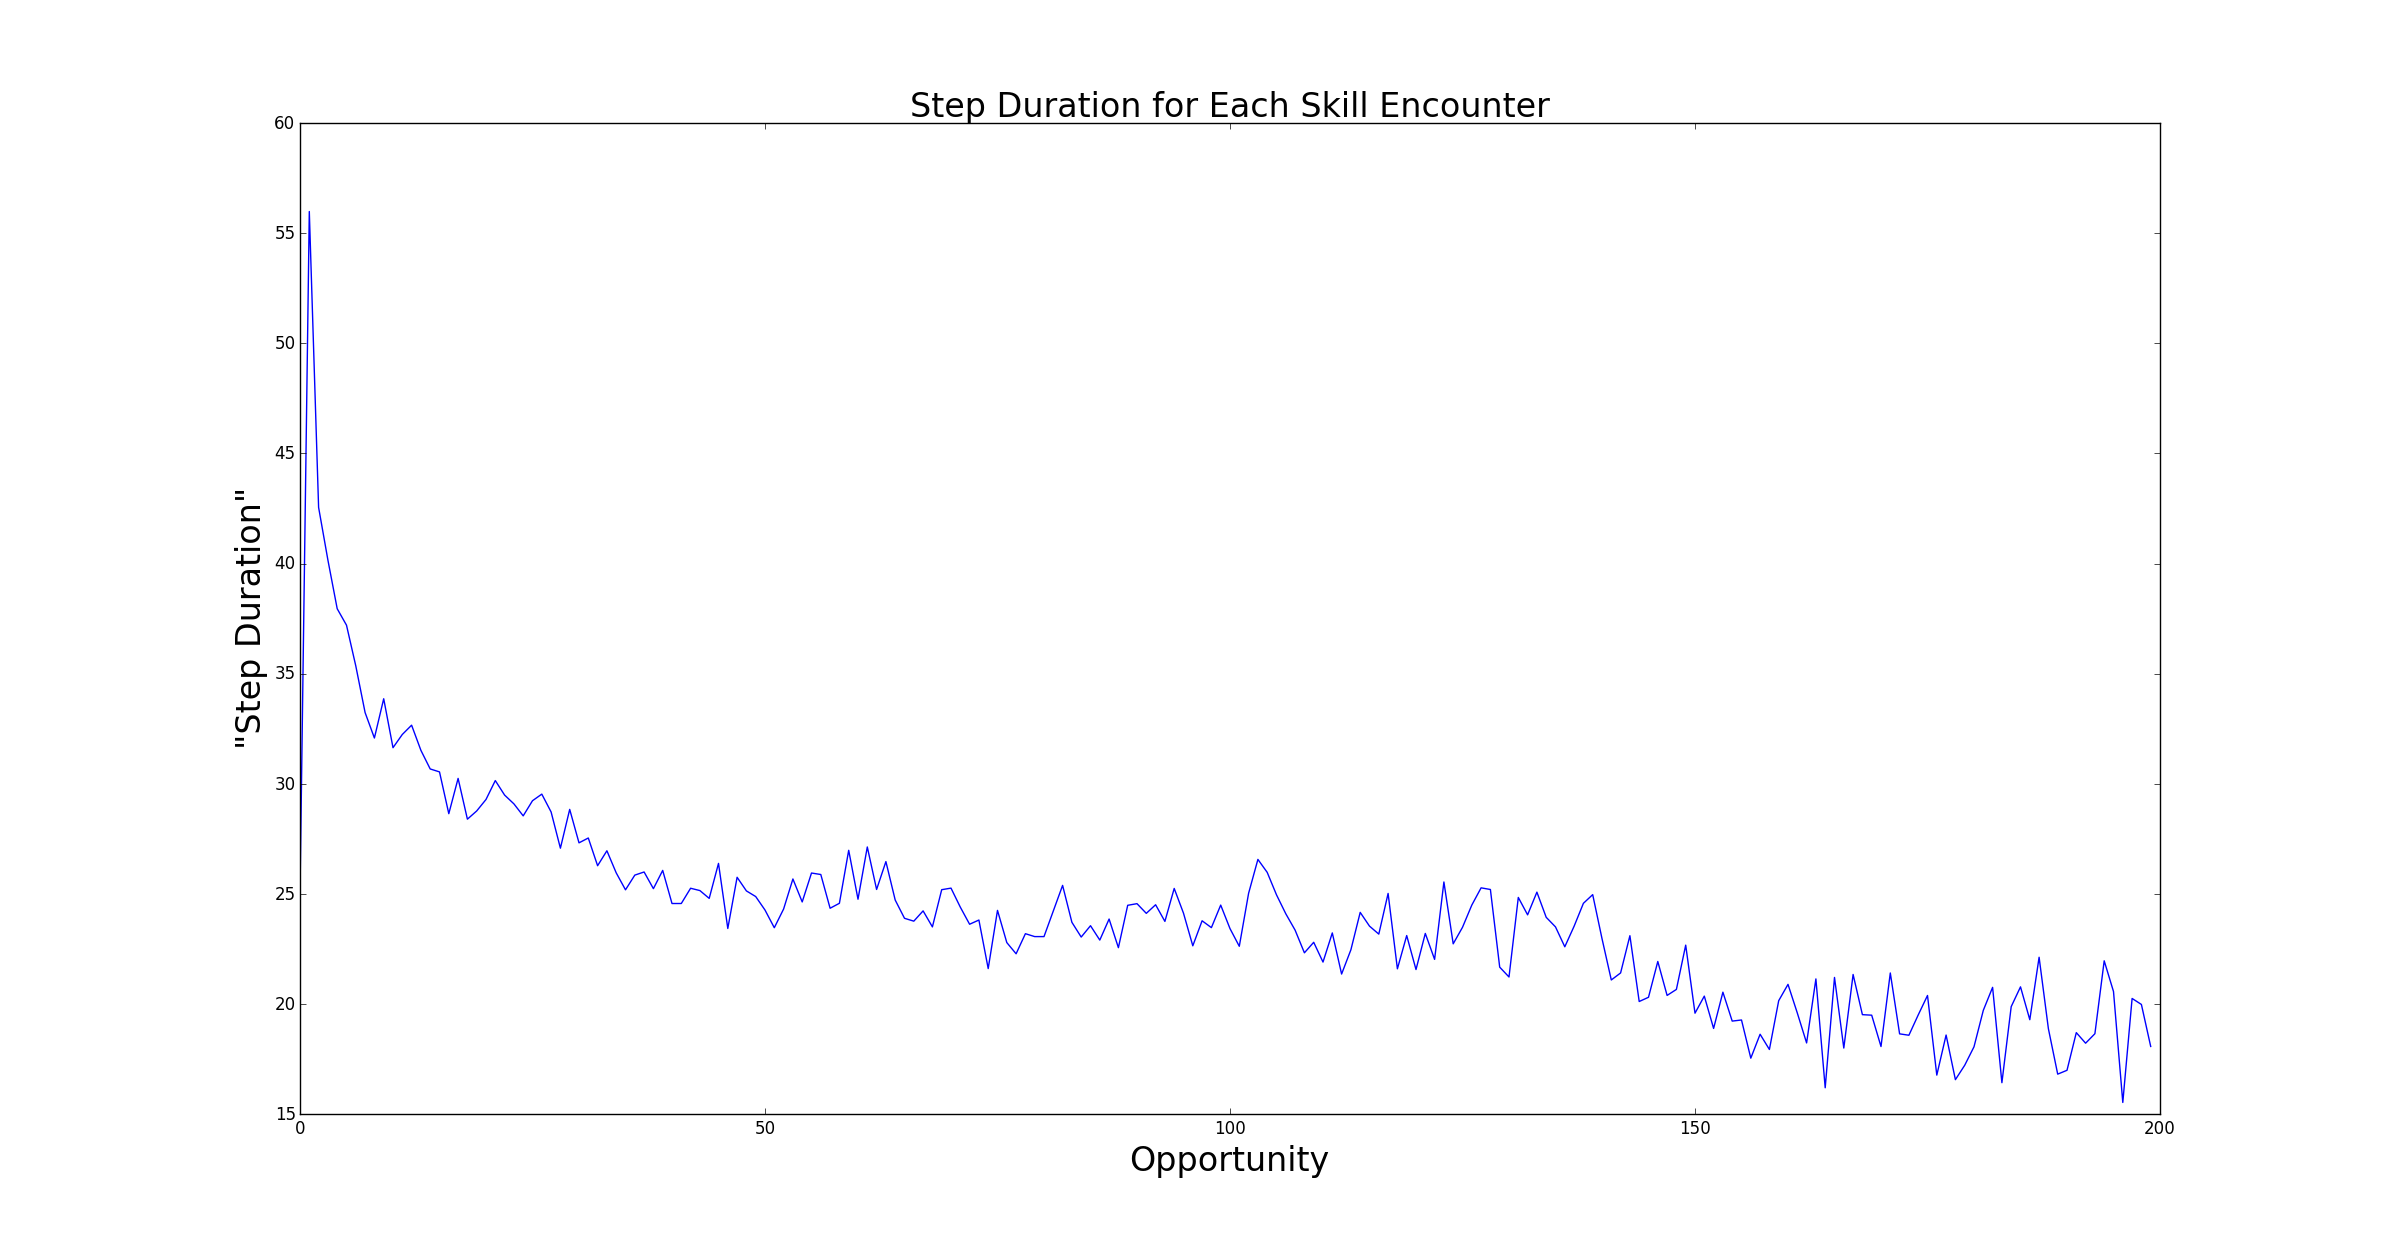
\includegraphics[width=0.8\textwidth]{stepdur_opp.png}
\label{stepdur}
\end{center}
\caption{"Step Duration" as a function of opportunity.}
\end{figure}


\begin{table}[t]
\begin{center}
\begin{tabular}{ccc|c|ccc|c|ccc}
\multicolumn{3}{c}{$\pi$} && \multicolumn{3}{c}{$T$} && \multicolumn{3}{c}{$E$}\\
S1 & S2 & S3 & & S1 & S2 & S3 && S1 & S2 & S3\\
& & & S1 & 0.096 & 0.654 & 0.25  &Empty & 0.010 & 0.0 & 0.0\\
0.56 & 0.328 & 0.112 & S2 & 0.004 & 0.972 & 0.024 &0-15s& 0.105 & 0.594 & 0.19\\
&&& S3 & 0.007 & 0.6 & 0.392 &15-30s& 0.202 & 0.149 & 0.595\\
&&&&&&&30-45s & 0.196 & 0.088 & 0.126\\
&&&&&&&45-60s & 0.045 & 0.051 & 0.014\\
&&&&&&&$>$60s& 0.442 & 0.122 & 0.067\\
\end{tabular}
\caption{Actual results from performing Stochastic Gradient Descent on the Baum-Welch algorithm.}\label{HMMprop}
\end{center}
\end{table}

In contrast to the template HMM shown in Table \ref{HMMprop}, we see from our Transmission matrix that we have a superfluous State 1 (the probabilities we transition to this state are shown in the first column of matrix $T$; all values are less than 0.1), and a terminal state 2. Comparing states 2 and 3, we see that it is more likely to have a shorter step duration in state 2 than in state 3. Apparently, state 3 is our "Unknowledgeable" state, while state 2 is our "Comprehension" state.

We then plug the output $\pi$, $T$, $E$ into the forward-backward algorithm to obtain $\gamma$, the probability we are in any of our states at a particular point in our history:
$$
\gamma_t(i) = \frac{\alpha_t(i)\beta_t(i)}{P(O|\lambda)}
$$
for all states $i$. Recall that $\alpha_t(i)$ measures the probability we are in state $i$ using data up to time $t$, while $\beta_t(i)$ measures the probability we are in state $i$ using date after time $t$, all normalized by the probability of the observed sequence given our values in $\pi$, $E$, and $T$. Thus, for any time point, we can determine the probability that an average student is either in the S3 ("Unknowledgeable") or S2 ("Comprehension") state.

With these given $\pi$, $T$, and $E$ matrices, 

\section{Conclusions}

The project gave us several insights into time allotment for a real-world type problem. Much of our time was spent trying to build these algorithms ourselves and test our functions which slowed down the process, but proved invaluable for comprehension of the methods and was somewhat fun. Additionally, a significant portion of the time was spent trying to understand the types of cases we could expect to see in the test data. We did not initially expect to find non-sequential questions in the test data relative to the training data, nor did we expect for their to be untracked students. So, a lot of time had to be allocated to parsing the data into a workable format, dealing with exceptions, and adjusting our plans for applying our HMM and decision tree. However, with all of that in mind, the vague strategy we started with was still able to be developed into a fitting plan.

We garnered one general idea applicable to other machine learning problems. In the situation where the test data has missing features an effective method is to generate similar features for the test data. In that way, an algorithm trained on the training data features can be applied to the test data. At the time of milestone our approach with the HMM was to generate an output at a subsequent time step of Correct First Attempt, which only yielded a guess slightly better than random. However, the best final results used the training data and HMM to predict a feature for the test data, Step Duration, that we knew to be fairly well correlated with the Correct First Attempt variable. We expect that generating more features in the test data would have yielded even better results. 

A couple additional ideas were proposed for extending the effectiveness of our methods. While our greatest succes came from predicting already tracked features of the data, e.g. step duration, we had also written a Viterbi algorithm which would have allowed us to track latent variables in the model between the training and test data. In fact, with the implementation of the Baum-Welch algorithm, had the freedom to generate many HMM's with different numbers of hidden states and  different combinations of observables. So, multiple numbers of models with varying hidden variable states could all have been generated and tracked over the training and test data. Interestingly, we see that through such an implementation, we lose the interpretations of the hidden variable states. A two or three state hidden variable no longer necessarily corresponds to student knowledge for example. We also somewhat underutilized the ''Knowledge Component skills'' provided due to the sparsity of individual skills over multiple students. These ideas ultimately required many more iterations of retraining and validating of the decision tree and HMM on components.


\subsubsection*{Acknowledgments}

Author JGL acknowledges Maximo Q. Menchaca for his quality work on the project described above. Author MQM acknowledges John G. Lee for his quality work on the project described above.

\subsubsection*{References}

\small{
[1] Frazzoli, E. (2010) Principles of Autonomy and Decision Making. 
\url{http://ocw.mit.edu/courses/aeronautics-and-astronautics/16-410-principles-of-autonomy-and-decision-making-fall-2010/lecture-notes/MIT16_410F10_lec21.pdf}\label{ref:hmmMIT}

[2] Domingos, P. (2015) \url{ http://courses.cs.washington.edu/courses/cse515/15wi/hmm.ppt}\label{ref:hmmUW}

[3] Lee, J.G.\& Menchaca, M.Q. (2015) Student Performance Prediction Using Hidden Markov Models and Decision Tree. CSE 546 Autumn 2015 Project Proposal, 1 pp., Unpublished.

[4] Guestrin, C. (2014) \url{ https://courses.cs.washington.edu/courses/cse546/14au/slides/decision-trees-annotated.pdf}

[5] Stamp, M. (2015) A Revealing Introduction to Hidden Markov Models \url{https://www.cs.sjsu.edu/~stamp/RUA/HMM.pdf}

[6] Lee, J.G.\& Menchaca, M.Q. (2015) Employing an HMM and Decision Tree to Predict Student Behavior. CSE 546 Autumn 2015 Milestone, 3 pp., Unpublished.

\end{document}